\documentclass{article}
	
\usepackage[margin=1in]{geometry}		% For setting margins
\usepackage{amsmath}				% For Math
\usepackage[]{amssymb}
\usepackage{amsmath}
\usepackage{gensymb}
\usepackage{fancyhdr}				% For fancy header/footer
\usepackage{graphicx}				% For including figure/image
\usepackage{cancel}					% To use the slash to cancel out stuff in work
\usepackage{wasysym}                % For cent symbol
\usepackage{needspace}              % To force item to next page

%%%%%%%%%%%%%%%%%%%%%%
% Set up fancy header/footer
\pagestyle{fancy}
\fancyhead[RO,R]{{\large\textbf{PHYS-102}}}
\fancyhead[LO,L]{\large{\textbf{Ch 17 Problem Set}}}
% \fancyhead[CO,C]{\large{\textbf{Part 1}}}
% \fancyhead[RO,R]{\today}
\fancyfoot[LO,L]{}
\fancyfoot[CO,C]{\thepage}
\fancyfoot[RO,R]{}
\renewcommand{\headrulewidth}{0.4pt}
\renewcommand{\footrulewidth}{0.4pt}
%%%%%%%%%%%%%%%%%%%%%%

\newcommand{\hmwkTitle}{Chapter 17 Temperature, Thermal Expansion, and Ideal Gas
Law}
% \newcommand{\hmwkDueDate}{February 12, 2014}
\newcommand{\hmwkClass}{PHYS-102}
% \newcommand{\hmwkClassTime}{}
% \newcommand{\hmwkClassInstructor}{Professor Isaac Newton}
\newcommand{\hmwkAuthorName}{\textbf{\underline{\hspace{3in}}}}

% math shortcuts
\newcommand\rr{\quad\Rightarrow\quad}

%
% Title Page
%

\title{
    \vspace{2in}
    \textmd{\textbf{\hmwkTitle}}\\
    \vspace{0.5in}
    \textmd{\textbf{\hmwkClass}}\\
    % \normalsize\vspace{0.1in}\small{Due\ on\ \hmwkDueDate\ at 3:10pm}\\
    % \vspace{0.1in}\large{\textit{\hmwkClassInstructor\ \hmwkClassTime}}
    \vspace{4in}
}

\author{\hmwkAuthorName}
\date{}
\begin{document}
\maketitle
\newpage
\begin{center}
    \section*{\textbf{\underline {Conceptual Questions}}}
\end{center}
\subsubsection*{
    1. Which has more atoms: 1 kg of iron or 1 kg of aluminum?
    See the Periodic Table or Appendix F. 
}
\subsubsection*{
    10. Figure 17–18 shows a diagram of a simple \textbf{thermostat} used
    to control a furnace (or other heating or cooling system). The
    bimetallic strip consists of two strips of different metals bonded
    together. The electric switch (attached to the bimetallic strip) is
    a glass vessel containing liquid mercury that conducts electricity 
    when it can flow to touch both contact wires. Explain how this device
    controls the furnace and how it can be set at different temperatures
}
\begin{figure}[h]
    \begin{center}
        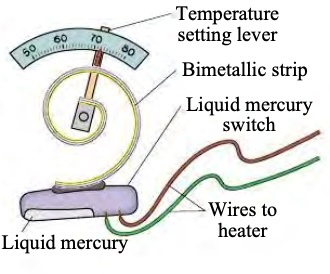
\includegraphics[width=0.4\textwidth]{figures/q10.jpg}
    \end{center}
\end{figure}
\subsubsection*{
    13. When a cold mercury-in-glass thermometer is first placed in a hot
    tub of water, the mercury initially descends a bit and then rises. Explain.
}
\newpage
\begin{center}
    \section*{\textbf{\underline {Problems}}}
\end{center}
\begin{center}
    \subsection*{\textbf{\textit{17-1 Atomic Theory}}}
\end{center}
\subsubsection*{
    1. How does the number of atoms in a 21.5-g gold ring compare to
    the number in a silver ring of the same mass? 
}
\begin{center}
    \subsection*{\textbf{\textit{17-2 Temperature and Thermometers}}}
\end{center}
\subsubsection*{
    3. (a) “Room temperature” is often taken to be 68°F. What is this
    on the Celsius scale? (b) The temperature of the filament in a lightbulb
    is about 1900°C. What is this on the Fahrenheit scale?
}
\begin{center}
    \subsection*{\textbf{\textit{17-4 Thermal Expansion}}}
\end{center}
\subsubsection*{
    7. The Eiffel Tower (Fig. 17–19) is built of wrought iron approximately 300 m
       tall. Estimate how much its height changes between January (average 
       temperature of 2°C) and July (average temperature of 25°C). Ignore the
       angles of the iron beams and treat the tower as a vertical beam
}
\begin{figure}[h]
    \begin{center}
        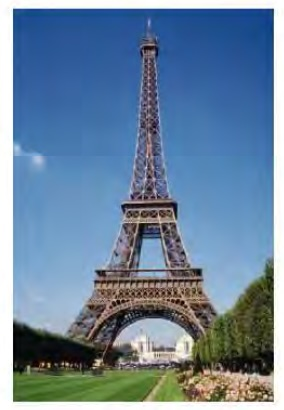
\includegraphics[width=0.2\textwidth]{figures/p7.jpg}
    \end{center}
\end{figure}
\subsubsection*{
    8. A concrete highway is built of slabs 12 m long (15°C). How wide should
    the expansion cracks between the slabs be (at 15°C) to prevent buckling if
    the range of temperature is –30°C to ±50°C?
}
\subsubsection*{
    17. It is observed that 55.50mL of water at 20°C completely fills a container
    to the brim. When the container and the water are heated to 60°C, 0.35 g of
    water is lost. (a) What is the coefficient of volume expansion of the container?
    (b) What is the most likely material of the container? Density of water at 60°C
    is 0.98324 g/mL.
}
\newpage
\begin{center}
    \subsection*{\textbf{\textit{17-7 and 17-8 Ideal Gas Law}}}
\end{center}
\subsubsection*{
    31. If 3.80 $m^3$ of a gas initially at STP is placed under a pressure of 3.20 atm,
    the temperature of the gas rises to 38.0°C. What is the volume?
}
\subsubsection*{
    34. If 14.00 mol of helium gas is at 10.0°C and a gauge pressure of 0.350 atm,
    calculate (a) the volume of the helium gas under these conditions, and (b) the
    temperature if the gas is compressed to precisely half the volume at a gauge
    pressure of 1.00 atm.
}
\subsubsection*{
    37. A storage tank at STP contains 28.5 kg of nitrogen ($N_2$). (a) What is
    the volume of the tank? (b) What is the pressure if an additional 25.0 kg
    of nitrogen is added without changing the temperature?
}
\subsubsection*{
    41. A sealed metal container contains a gas at 20.0°C and 1.00 atm. To what
    temperature must the gas be heated for the pressure to double to 2.00 atm? 
    (Ignore expansion of the container.)
}
\subsubsection*{
    44. A helium-filled balloon escapes a child’s hand at sea level and 20.0°C.
    When it reaches an altitude of 3600 m, where the temperature is 5.0°C and
    the pressure only 0.68 atm, how will its volume compare to that at sea level?
}
\subsubsection*{
    50. An air bubble at the bottom of a lake 37.0 m deep has a volume of
    1.00 $cm^3$. If the temperature at the bottom is 5.5°C and at the top
    18.5°C, what is the volume of the bubble just before it reaches the surface?
}
\begin{center}
    \subsection*{\textbf{\textit{17-9 Ideal Gas Law in Terms of Molecules;
    Avogadro's Number}}}
\end{center}
\subsubsection*{
    51. Calculate the number of $\frac{molecules}{m^3}$ in an ideal gas at STP.
}
\subsubsection*{
    52. How many moles of water are there in 1.000 L at STP? How many molecules?
}
\newpage
\begin{center}
    \subsection*{\textbf{\textit{General Problems}}}
\end{center}
\subsubsection*{
    69. A house has a volume of $870\;m^3$. (a) What is the total mass of air inside
    the house at 15°C? (b) If the temperature drops to –15°C, what mass of air
    enters or leaves the house?
}
\end{document}
